\documentclass{acm_proc_article-sp}
\usepackage{wrapfig}
\usepackage{tikz, alex, url, mu}
\usetikzlibrary{arrows,shapes,snakes,automata,backgrounds,petri}
\tikzset{>=stealth}

\title{Quilting for Distributed Machine Learning System}

\author{Mu Li \\ CMU CSD \and Jinliang Wei\\ CMU CSD}

\begin{document}
\maketitle

\begin{abstract}
In this paper we proposal QuiltDB, a distributed database optimized for network
topology.
\end{abstract}

\section{Introduction}

In distributed machine learning applications, data as well as computation are
partitioned among hundreds or  thousands of machines. Those
worker machines compute local results based on their own data. Global solutions
are then obtained via synchronization.

Machine synchronization, including data communication and waiting, is typically
the most expensive operation, because of limited network bandwidth and highly
variant machine performances. Recently, asynchronous communication is proposed
to hide the synchronization cost, however, those works assume the network has
uniform point-to-point bandwidth.

However, the real data datacenter network usually has specially topology. For
example, machines are grouped by ranks, and those ranks are then connected by
several layers of switchers. It thus forms a (multi-)tree like
topology. Machines within a rack has much larger bandwidth than crossing racks.

It is necessary to consider the network topology, because of the huge amount of
data communication volume and iterative nature of  machine learning
applications. In addition, if the communication forms a simple pattern, such as
a ring or a start, then it is much easier to improve the machine network
according this to pattern than improve the overall point-to-point bandwidth.

On this paper, we propose a database execute engine, QuiltDB, which mapping
machine learning applications into network topologies. Key features of this
system includes,

\begin{itemize*}
\item Allow use-defined network topology.
\item Model machine learning applications by the primal-dual decomposition.
\item A discrete streaming system.
\end{itemize*}

\section{Network Topologies}
\label{sec:network-topologies}

Several network topologies have been proposed by HPC community, including grid,
hyper-cube, buffer-fly, etc. Algorithms are then mapped into network topology to
maximize the communication efficiency. On the other hand, cloud computing
typically adopts
tree-like structures, which aims to approximate an uniform all-to-all connection
and provide fault tolerance and elastic scalability.

\subsection{Grid Communication}

Grid is the one of the simplest communication pattern, which is shown in
Figure~\ref{fig:grid2}. Machines are connected both vertically and
horizontally. Each machine only communicates with its 4 neighbors. Its
restricted connections make it comparable cheap to build the physical
network. It also relieves switchers' burden on the cloud computing setting.
However, if the two machines are far away, then the network delay between these
two is also large.


\begin{figure}[th!]
  \centering
  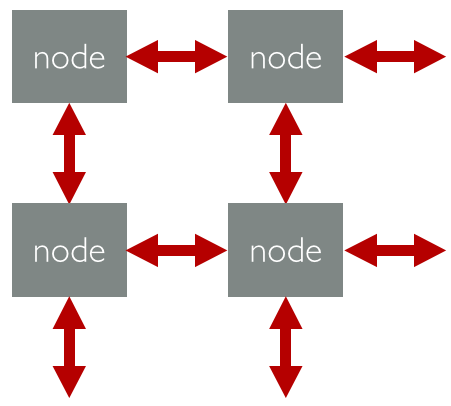
\includegraphics[width=.25\textwidth]{fig/grid}
  \caption{Grid communication}
  \label{fig:grid2}
\end{figure}


\subsection{Two-layer Network}

The grid communication is somewhat too restrictive. Nowadays machines within a
datacenter are typically first connected by top-rack switchers. Due to the high
bandwidth in a switcher, machines in the same rack usually have decent
point-to-point bandwidth. Therefore we may use more flexible within rack
communication pattern. Figure~\ref{fig:rack} shows a simple example, where
machines only talk to the others in the neighbor rack, while any two machines
within the same rack could communicate.
\begin{figure}[th!]
  \centering
  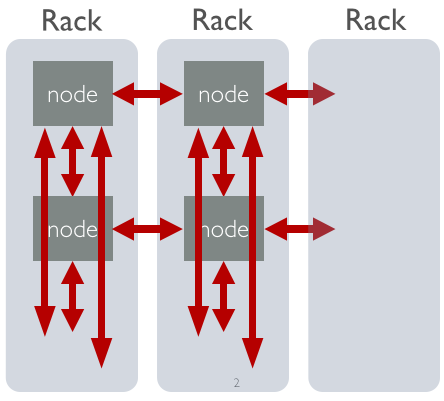
\includegraphics[width=.25\textwidth]{fig/rack}
  \caption{More flexible within rack communication.}
  \label{fig:rack}
\end{figure}

\section{Machine Learning Applications}

On this section, we describe several machine learning applications which fits
into the communication pattern we discussed on Section
\ref{sec:network-topologies}.

\subsection{Data Partition}

On a typical distributed machine learning application, both data and shared
parameters are partitioned into a group of machines.
Different partitioning scheme requires different amount of data to be
communicated. For example, consider the following iterative matrix
multiplications, which is a typical machine learning workload:
\begin{align*}
w &= X u \\
u &= X^T w,
\end{align*}
where $X$ is a gigantic data matrix and $u$ and $w$ are two vectors.

Given a $n$-by-$m$ matrix $X$, we want to divide the matrix into $p$ machines
while minimizing the amount of data to be communicated in each iteration.

If we cut the matrix into $a$ rows and $b$ columns, then the minimal data
communication is

\begin{equation}
  r  am +  c bn
  \label{eq:total-traffic}
\end{equation}
where $r,c \in [0,1]$ are coefficient depending on the sparsity of the
matrix. They should be a function as $a$ and $b$, but now we consider it as a
constant to simply the calculation.

Note that $ab=p$, then (\ref{eq:total-traffic}) get minimize value when
$a = \rbr{ \frac{cn}{rm} }^{\frac{1}{2}}\sqrt{p}$. That is, if $cn \gg rm$, we
should choose partition scheme 1, if $rm \gg cn$, we should use scheme 2, while
if $rm \approx cn$, the even partition scheme 3 is a better choice.

\begin{figure}[th!]
  \centering
\begin{tikzpicture}[scale=.5]
  \draw [fill=set12!60](0,0) rectangle (4,1)
  rectangle (0,2) rectangle (4,3) rectangle (0,4);
  \draw[xshift=6cm, fill=set11!60] (0,0) rectangle (1,4) rectangle (2,0) rectangle (3,4)
  rectangle (4,0);
  \draw[xshift=12cm, fill=set13!60] (0,0) rectangle (2,2) rectangle (0,4);
  \draw[xshift=14cm, fill=set13!60] (0,0) rectangle (2,2) rectangle (0,4);
\end{tikzpicture}
  \caption{partition scheme 1 to 3: $a=4,b=1$, $a=1,b=4$, and $a=2,b=2$}
\end{figure}

\subsection{Pagerank}

Given adjacent matrix $X$, where $X_{ij} = 1 $ if and only if webpage $i$ cites
$j$. Denote by $D=\textrm{diag}{\sum_i X_{i1}, \ldots, \sum_{i=1} X_{in}}$ the diagnal
adjacent matrix, then pagerank can be solved by.
\begin{equation}
  w = \alpha X^T D^{-1} w + (1-\alpha)\frac{1}{n}
\end{equation}

\begin{figure}[th!]
  \centering
  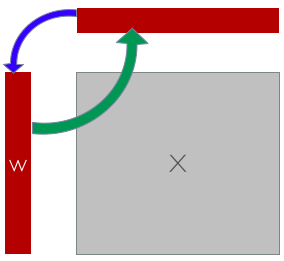
\includegraphics[width=.25\textwidth]{fig/pr}
  \caption{Pagerank}
  \label{fig:pr}
\end{figure}

The workload is summarized in Figure~\ref{fig:pr}. It is convenient to view the
updating as two steps, the
first step compute the new value of $w$, and then update $w$. To extend pagerank
into a distributed algorithm, we consider the grid data partition. Then each
machine also execute the computing and then updating steps. The only difference
is that updating involves network communications. On the example, each rack get
a group of columns of $X$. One particular  machine in the rack gathers the
updates within the rack and then propagates to other racks.

\begin{figure}[th!]
  \centering
  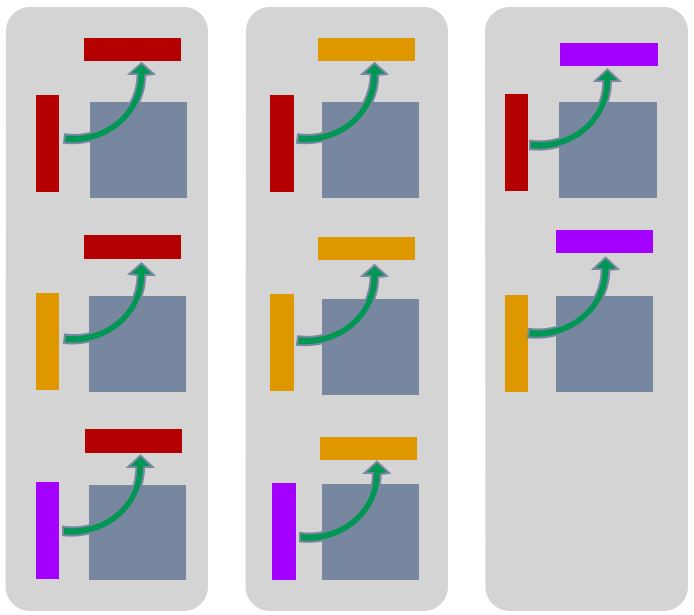
\includegraphics[width=.25\textwidth]{fig/compute}
  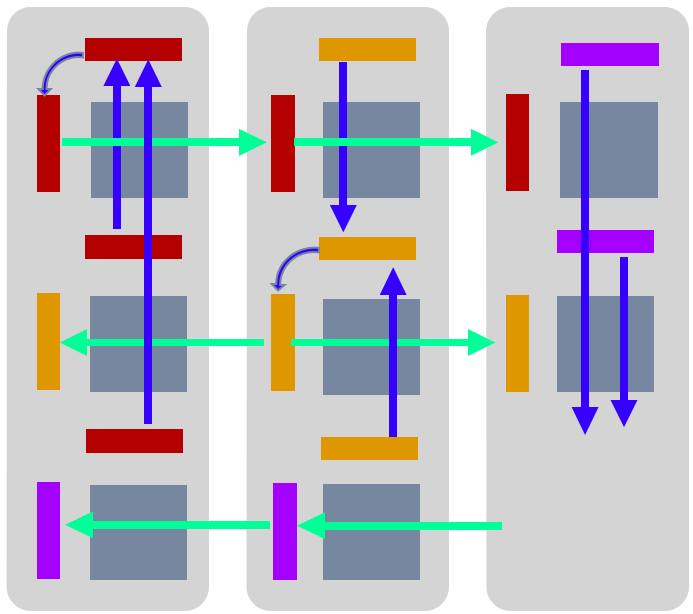
\includegraphics[width=.25\textwidth]{fig/update}
  \caption{Two steps of pagerank: compute and then update}
\end{figure}

\subsection{Loss minimization}

Loss minimization solves the following optimization problem:
\begin{equation}
  \min_w \sum_{i=1}^{n} f(\langle x_i, w\rangle, y_i) + \lambda r(w)
\end{equation}
It fits into our setting by considering the primal-dual view, where $w$ is the primal
variable, while $\partial f(\langle x_i, w\rangle, y_i) x_i$ is the dual. Then
the optimization method computes and updates the prime and dual alternatively.


\section{Implementation}

\section{Experiments}

\subsection{Setup}


\appendix


\appendix
\section{Acknowledgements}
The authors would like thank to Alex Smola, Dave Andersen (potentially more...)
for helpful discussion.

\bibliography{ref}
\bibliographystyle{abbrvnat}

\end{document}
